\documentclass{standalone}
\usepackage{tikz}
\usetikzlibrary{shapes,arrows,calc,positioning,decorations.markings,shadows}
\usepackage{amsmath,amsfonts,graphicx,pgfplots}
\begin{document}
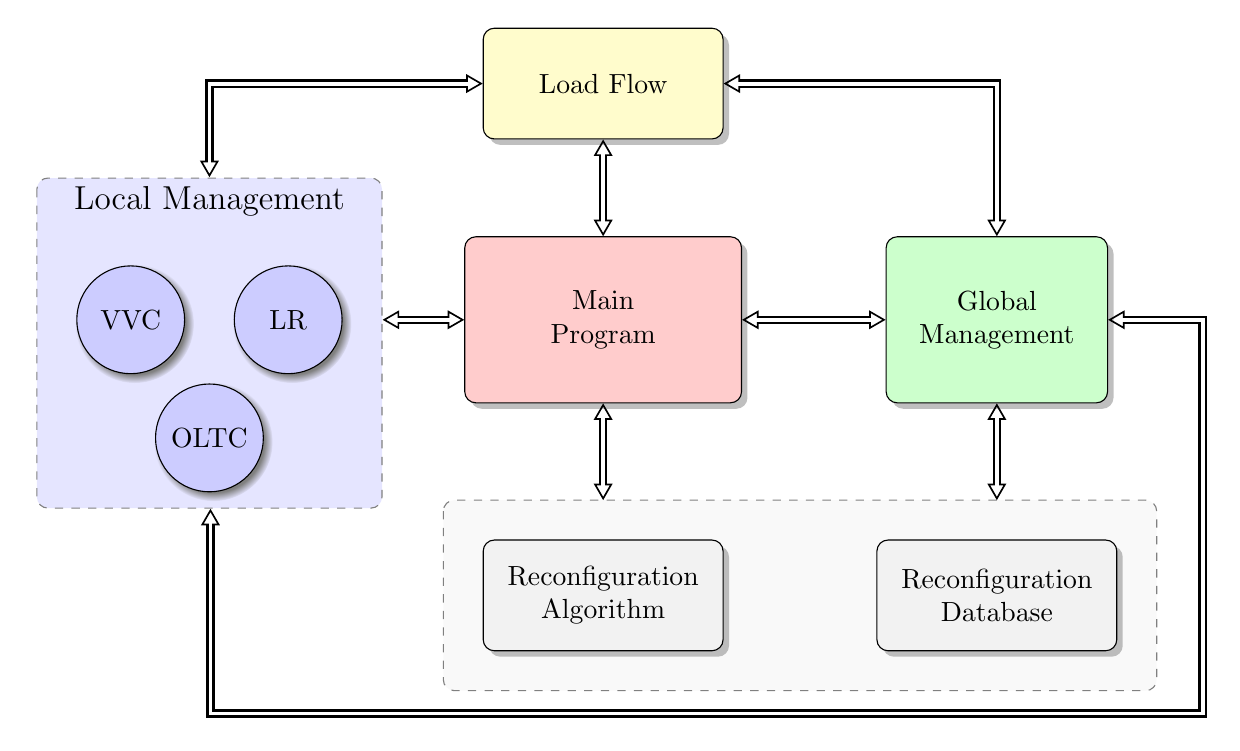
\begin{tikzpicture}

    \pgfdeclarelayer{background}
    \pgfdeclarelayer{foreground}
    \pgfsetlayers{background,main,foreground}

    \tikzstyle{lcomp}=[draw, fill=blue!20, text width=5em, 
        text centered, minimum height=2.5em,text centered]

    \tikzstyle{ann} = [above, text width=5em]

    \tikzstyle{program} = [lcomp, text width=6em, fill=red!20, 
        minimum height=6em, minimum width=10em, rounded corners,text centered, drop shadow]

    \tikzstyle{global} = [lcomp, text width=6em,
        fill=green!20, minimum height=6em, minimum width=8em, rounded corners,text centered, drop shadow]

    \tikzstyle{reconf} = [lcomp, text width=8em, fill=gray!10, 
        minimum height=4em, minimum width=8em, rounded corners,text centered, drop shadow]

    \tikzstyle{lf} = [lcomp, text width=8em, fill=yellow!20, 
        minimum height=4em, minimum width=8em, rounded corners,text centered, drop shadow]

    \tikzstyle{local} = [draw, circle, text width=3em, fill=blue!20,
        minimum height=3em, minimum width=3em, text centered, circular drop shadow]

    \tikzstyle{blank} = [node distance=1cm,minimum width=-1cm]

    \tikzstyle{vecArrow} = [thick, decoration={markings,mark=at position 0 with {\arrowreversed[semithick]{open triangle 60}},mark=at position
       1 with {\arrow[semithick]{open triangle 60}}},
       double distance=1.4pt, shorten >= 5.5pt, shorten <= 5.5pt,
       preaction = {decorate},
       postaction = {draw,line width=1.4pt, white,shorten >= 4.5pt, shorten <= 4.5pt}]
    \tikzstyle{innerWhite} = [semithick, white,line width=1.4pt, shorten >= 4.5pt, shorten <= 4.5pt]


	% Main Program
    \node [program] (prog) {Main Program};

    % Reconfiguration
    \node [blank,right of=prog, node distance=1cm] (b1) {};
    \node [reconf,below of=prog, node distance=3.5cm] (rec) {Reconfiguration Algorithm};
    \node [reconf, right of=rec,node distance=5cm] (recdb) {Reconfiguration Database};
    \node [blank, left of=rec, node distance=2cm] (b5) {};

    % Load Flow
    \node [lf, above of=prog, node distance=3cm] (ld) {Load Flow};

    % Local Management
    \node [blank, below of=prog, node distance=3cm] (b2) {};
    \node [local, left of=prog, node distance=4cm] (lr) {LR};
    \node [local, left of=lr, node distance=2cm] (vvc) {VVC};
    \node [blank, left of=lr, node distance=1cm] (b3) {};
    \node [blank, right of=lr, node distance=1cm] (b4) {};
    \node [local, below of=b3, node distance=1.5cm] (oltc) {OLTC};
    \node [blank, above of=oltc, node distance=3cm] (lmg) {\large Local Management};

    % Global Management
    \node [global,right of=prog, node distance=5cm] (gm) {Global Management};

    \begin{pgfonlayer}{background}
        \path (vvc.west)+(-0.5,1.8) node (a) {};
        \path (oltc.south -| lr.east)+(+0.5,-0.2) node (b) {};
        \path[fill=blue!10,rounded corners, draw=black!50, dashed]
            (a) rectangle (b);

        \path (rec.north west)+(-0.5,0.5) node (c) {};
        \path (recdb.south east)+(+0.5,-0.5) node (d) {};
        \path[fill=gray!05,rounded corners, draw=black!50, dashed]
            (c) rectangle (d);
    \end{pgfonlayer}

    \draw[vecArrow] (prog.north)+(0,0) to (ld);
    \draw[innerWhite] (prog.north)+(0,0) to (ld);

    \draw[vecArrow] (lmg.north)+(0,0) |- (ld);
    \draw[innerWhite] (lmg.north)+(0,0) |- (ld);

    \draw[vecArrow] (gm.north)+(0,0) |- (ld);
    \draw[innerWhite] (gm.north)+(0,0) |- (ld);

	\draw[vecArrow] (b4)+(0.2,0) to (prog);
    \draw[innerWhite] (b4)+(0.2,0) to (prog);

    \draw[vecArrow] (prog.east)+(0,0) to (gm);
    \draw[innerWhite] (prog.east)+(0,0) to (gm);

	\draw[vecArrow] (rec.north)+(0,0.5) to (prog.south);
    \draw[innerWhite] (rec.north)+(0,0.5) to (prog.south);

    \draw[vecArrow] (recdb.north)+(0,0.5) to (gm.south);
    \draw[innerWhite] (recdb.north)+(0,0.5) to (gm.south);

    \draw[vecArrow] (gm.east)+(0,0) to node {} +(1.2,0) to node {} +(1.2,-5) to node {} +(-11.4,-5) to node {} +(-11.4,-2.4);
    \draw[innerWhite] (gm.east)+(0,0) to node {} +(1.2,0) to node {} +(1.2,-5) to node {} +(-11.4,-5) to node {} +(-11.4,-2.4);
    
\end{tikzpicture}
\end{document}